\chapter{Machine Learning}

In the world of data science there are two main views. From one side there is the mathematically well founded statistical methods like \textbf{statistical learning\index{statistical learning}} which mainly focuses on explaining population data from a sample. Various linear models are well defined within statistics. \textbf{Machine learning\index{Machine learning}} contains more complex techniques which might not have well founded probabilistic interpretations but provide good empirical results. There is major overlap and no easy way to differentiate the two views. We will start from statistical learning and move toward more complex machine learning models.

The most important building block of machine learning is the concept of a \textbf{model\index{model}}. A model is a series of assumptions or a simplified representation of a system. A model can be one or multiple mathematical equations, accompanied by a set of assumptions. The model might also be called a \textbf{data generator process\index{data generator process}} because based on the assumptions and simplifications it can generate new data with some error (see below).

In machine learning we try to fit a \textbf{model\index{model}} to a data set. There are two main objectives why we would like to do this:

\begin{itemize}
    \item \textbf{Inference\index{Inference}} about population properties by calculating the model properties.
    \item \textbf{Forecast\index{Forecast}} values of the population outside of the available sample/observations
\end{itemize}

The variable we would like to model or forecast is called the \textbf{dependent\index{dependent}} variable. The input variables used for modelling or forecast are called \textbf{independent\index{independent}} variables. We can model an \textbf{dependent\index{dependent}} \(Y\) variable with the \textbf{independent\index{independent}} variables \(X\) of a sample of observations. We assume the following relationship between the variables

\begin{equation}Y = f(X) + \epsilon \tag{4.1}\end{equation}

We define a model in the form

\begin{equation}\hat{Y} = \hat{f}(X) \tag{4.2}\end{equation}

\(\epsilon\) is the error term and can be decomposed using the expected value of (4.1) and (4.2) to two terms, called the \textbf{reducible error\index{reducible error}} and the \textbf{irreducible error\index{irreducible error}}:

\[E[(Y-\hat{Y})^2] = \underbrace{[f(X)-\hat{f}(X)]^2}_\text{Reducible error} + \underbrace{\text{Var}(\epsilon)}_\text{Irreducible error}\]

Proof:
\begin{flalign*}
& \text{Using (4.1) and (4.2)} \\
& E[(Y-\hat{Y})^2]=E[(f(X)+\epsilon-\hat{f}(X))^2] \\
& =E[(f(X)-\hat{f}(X))^2+2 \epsilon (f(X)-\hat{f}(X)) +\epsilon^2] \\
& \text{Because the expectation is linear operator} \\
& =E[(f(X)-\hat{f}(X))^2] +2E[\epsilon (f(X)-\hat{f}(X))] +E[\epsilon^2] \\
& \text{Because the expectation of} f \text{and} \hat{f} \text{are constant} \\
& =[f(X)-\hat{f}(X)]^2 +E[\epsilon^2] +2E[\epsilon (f(X)-\hat{f}(X)) \\
& \text{Because the mean of} \epsilon \text{is zero} \\
& =[f(X)-\hat{f}(X)]^2 +E[\epsilon^2] \\
& \text{Because the variance of} \epsilon \text{is} E(\epsilon^2) \\
& =[f(X)-\hat{f}(X)]^2 + \text{Var}(\epsilon) \\ && \end{flalign*}

We can optimize our model to minimize the reducible error but irreducible error is also unknown and our model might overfit by including some fit on the noise as well.

In many cases we need to assume casual relationship such as X causes Y, but in fact in some cases might be the opposite direction.

\section{Estimators}

An \textbf{estimator\index{estimator}} is a function of the data. It can either estimate parameters of the data directly or we can use it to estimate model parameters to find the best fit of the model to the data. Depending on the output of estimator we distinguish the following types of estimators:

\begin{itemize}
    \item \textbf{Point estimator\index{Point estimator}}: outputs a single value for a parameter. It is easy to interpret but might not give information on the variability or confidence.
    \item \textbf{Interval estimator\index{Interval estimator}}: outputs an interval providing insight to the confidence of the output.
    \item \textbf{Bayesian estimator\index{Bayesian estimator}}: outputs a probability distribution.
\end{itemize}

Given a population parameter \(\beta^P\), an estimator function \(\hat \beta\),and the samples \(S_1, S_2, ..., S_n\), we can apply the estimator function to each sample. This would result in a set of estimated parameters \(\beta^*_1, \beta^*_2, ..., \beta^*_n\)


\begin{figure}[htbp]
    \begin{center}
        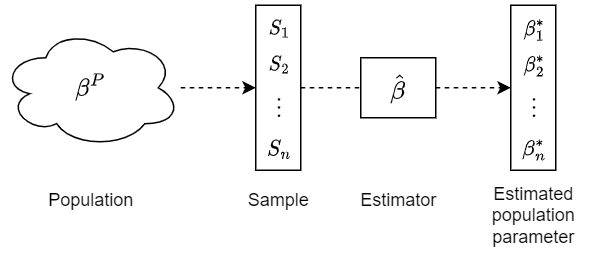
\includegraphics[width=250pt]{../img/03-estimator.png}
        \caption{Figure 3.1: Applying estimator to a set of observations}
    \end{center}
\end{figure}


Since the samples might not be fully representative of the population, the estimated parameters might also have some error to the real parameter \(\beta^P\).

If we calculate a property of multiple or all samples like the mean or variance these are also estimators for properties of the population.

We can define the following characteristics of an estimator

\begin{enumerate}
    \item \textbf{Unbiased\index{Unbiased}}: The expectation (mean) of the estimator matches the population parameter it estimates (see \textbf{Figure 3.2\index{Figure 3.2}} where the mean of the distribution is equal to the true population parameter)
\end{enumerate}

\[E[\hat \beta] = \beta^P\]

\begin{enumerate}
    \item \textbf{Consistent\index{Consistent}}: As the sample size grows, the estimator tends to the true value of the parameter (see \textbf{Figure 3.2\index{Figure 3.2}} where the red line is a small sample, the blue line is a larger sample and the green line would be an infinitely large sample or the entire population)
\end{enumerate}

\[n \to +\infty: \hat \beta \to \beta^P \]


\begin{figure}[htbp]
    \begin{center}
        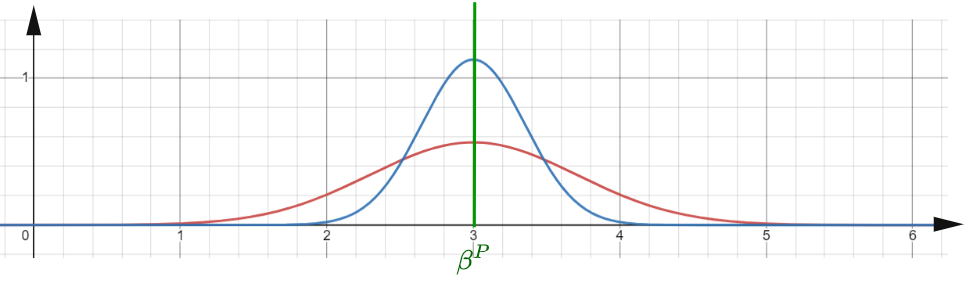
\includegraphics[width=250pt]{../img/03-estimate-distribution.png}
        \caption{Figure 3.2: <i>Plot of the probability distribution for the estimates which we get by applying an unbiased and consistent estimator to each sample. The red distribution is for a smaller sample with higher variance, the blue one is less variance measured on higher sample.</i>}
    \end{center}
\end{figure}


\textbf{Figure 3.3\index{Figure 3.3}} shows a biased but consistent estimator. For small sample sizes there is a bias between the true parameter and the mean of estimated parameters, but as the sample size increases, the distribution tends toward the true parameter.



\begin{figure}[htbp]
    \begin{center}
        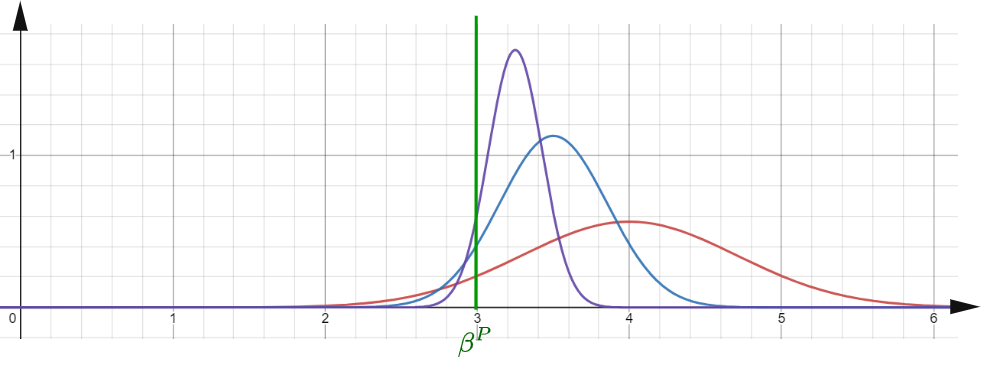
\includegraphics[width=250pt]{../img/03-biased-consistent-estimator.png}
        \caption{Figure 3.3: <i>Biased consistent estimator.</i>}
    \end{center}
\end{figure}



\begin{enumerate}
    \item \textbf{Efficiency\index{Efficiency}}: given two estimators \(\hat \beta\) and \(\widetilde \beta\), the estimator \(\widetilde \beta\) is said to be more efficient if it has lower variance using the same sample size. An efficient estimator might be biased. An example would be in \textbf{Figure 3.2\index{Figure 3.2}} if it were two different estimators with same sample size, one of them giving a more accurate distribution.
\end{enumerate}

\begin{enumerate}
    \item \textbf{Linear in parameters\index{Linear in parameters}} might be preferable so it can be mathematically easily manipulated.
\end{enumerate}

A specific case are the so called \textbf{BLUE estimators\index{BLUE estimators}} which stands for \textbf{best linear unbiased estimators\index{best linear unbiased estimators}}, meaning there is no better linear estimator available.

\section{Model fitting}

There are two main probabilistic optimization frameworks to estimate model parameters, also called \textbf{weights\index{weights}} in machine learning, given a set of observations: \textbf{Maximum Likelihood Estimation\index{Maximum Likelihood Estimation}} (MLE) and \textbf{Maximum a Posteriori\index{Maximum a Posteriori}} (MAP). The difference is that MAP assumes a prior probability distribution and tries to estimate parameters using the posterior probability, MLE estimates parameters using the prior based on observations only.

\[\theta_{MLE} = argmax_{\theta}\ f_n(x_1...x_n|\theta)\]

If values of \(x_1...x_n\) are i.i.d or we assume it, becomes

\[\theta_{MLE} = argmax_{\theta}\ \prod_{i=1}^nf(x_i|\theta)\]

We than try to optimize \(L(\theta)\). Since it's an optimization problem, we can optimize log likelihood of \(log\ L(\theta)\) instead to facilitate derivative calculations and avoid underflow due to several products of small decimal values.

If we assume a prior distribution in addition to our observations, we can apply MAP, which maximizes the posterior function :

\[
\begin{aligned}
\theta_{MAP} &= argmax_{\theta}\ f(\theta|x_1...x_n) \\
&= argmax_{\theta}\ g(\theta) f(x_1...x_n|\theta)
\end{aligned}
\]

We skipped the denominator (so-called marginal likelihood) after applying the Bayes rule above because it does not change the optimization problem.

For example for linear regression, MLE estimates the mean squared loss, applying MAP will estimate L2 regularization as well.

There are two main methods of model fitting
\begin{itemize}
    \item If there is closed solution for the optimization we can apply analytical calculation. This is only possible in few cases, for simple models with few parameters
    \item Iterative approach: a more commonly used approach, which can fit very complex models
\end{itemize}

\section{Cost function and bias-variance trade-off}

To measure how well the model fits our observed data we can use a \textbf{cost function\index{cost function}}. For a function to be considered as a cost function, it needs to fulfill the following attributes

\begin{itemize}
    \item Should always be positive
    \item If our estimate improves, the cost function should decrease
\end{itemize}

Using the likelihood function, which is the probability we can observe our data given our model, we can transform it to be a positive function, which decreases the better the fit. This is called the \textbf{negative log likelihood cost function\index{negative log likelihood cost function}}. Given a set of observations \(X\) and a statistical model with parameters \(\theta\) and the likelihood \(L(\theta | X)\), the cost function is:

\[\operatorname{NLL} = - \ln(L(\theta | X))\]

This equation looks scary, but likelihood is basically the probability of observing the data given the model parameters. The logarithms is used because it provides several computational benefits:

\begin{itemize}
    \item Since probabilities are usually small numbers. When multiplied together, as in the case of joint probabilities for sequences, they can become extremely small and lead to underflow issues in computers (since computers can store numbers up to some precision, the value might become smaller than this precision, leading to instability).
    \item In many cases, especially when working with likelihoods, products of probabilities get converted to sums when we take the logarithm. This transformation simplifies the computations and makes them more efficient. For example \(\log(p_1  p_2) = \log(p_1) + \log(p_2)\)
\end{itemize}

The likelihood function is mainly used to estimate parameters of probability distribution given the observed data, but might not have closed form or might have more than one local minima which is why other cost functions which are easier to optimize might be used to fit machine learning models.

A popular example of a cost function is the \textbf{mean squared error\index{mean squared error}} or MSE, which is the average of the squared difference of predicted and actual output for each observation \(i\).

\[\operatorname{MSE} = {1 \over n} \sum_{i=1}^n(y_i - \hat{f}(x_i))^2 \]

The MSE of an estimator \(\hat{\theta}\) with respect to an unknown parameter \(\theta\) is defined as

\[\operatorname{MSE}(\hat\theta)=E_\theta[ ({\hat \theta}-\theta )^{2} ]\]

MSE can be decomposed to a combination of bias and variance of the estimator

\[{\displaystyle \operatorname {MSE} ({\hat \theta})=\operatorname {Var} _\theta({\hat \theta})+\operatorname {Bias} ({\hat \theta},\theta )^{2}}\]

Proof

Using the definition of variance
<!--mleq-->
\(\operatorname{Var}(X) = E(X^{2}) - (E(X))^{2}\) \\
\(E(X^{2})=\operatorname{Var}(X)+(E(X))^{2}\)

By substituting \(X\) with \(\hat {\theta }-\theta\) it can be shown that

\(\operatorname{MSE} ({\hat {\theta }})=\mathbb {E} [({\hat {\theta }}-\theta )^{2}]\)\\
\(=\operatorname {Var} ({\hat {\theta }}-\theta )+(\mathbb {E} [{\hat {\theta }}-\theta ])^{2}\)\\
\(=\operatorname {Var} ({\hat {\theta }})+\operatorname {Bias} ^{2}({\hat {\theta }})\)
<!--mleq-->

Variance is always positive and bias is squared. The selected estimator needs to minimize either of or both of variance and bias in order to minimize \(\operatorname{MSE}\)

We can scale MSE to be the same size as our data, this metric is called \textbf{Root Mean Square Error\index{Root Mean Square Error}} or RMSE

\[\operatorname{RMSE} = \sqrt{\operatorname{MSE}}\]

For other cost functions we don't have a neat mathematical decomposition like with MSE, we still observe a tradeoff. For various other loss functions, the essence of the bias-variance tradeoff still exists. Whether we are using cross entropy for logistic regression, or custom loss functions for other models, the fundamental tension between fitting the training data well (and risking overfitting) versus generalizing to new data (and risking underfitting) remains. A model with too many parameters might overfit the training data and perform poorly on new, unseen data (high variance, low bias). Conversely, an overly simple model might not capture the underlying patterns in the training data, leading to systematic errors (high bias, low variance).

\section{Regularization}

\section{Model selection}

When we would like to fit a model to the data. We first assume a model structure, this process is called \textbf{model selection\index{model selection}} e.g. a linear model, tree model, neural network, etc. Many of the models have some assumptions about the data we try to fit the model to. We need to consider or verify these assumptions. When selecting a model we also consider difficulty of building. Some models can be created more easily (e.g linear models, tree models) compared to others which require more work (neural network).

Once we selected our model, we proceed to estimate the model parameters. There are two main types of model parameters:
\begin{itemize}
    \item \textbf{Weights\index{Weights}} or \textbf{parameters\index{parameters}}: are function parameters we can adjusted during the learning process to best fit the model to the observed data.
    \item \textbf{Hyperparameters\index{Hyperparameters}}: describe the structure of model or method of model fitting, e.g. learning rate, layers in a neural network, the K in KNN, etc
\end{itemize}

The methods of estimating weights and the methods of finding the right hyperparameters are different.

\section{Model validation}

Cross validation
Goodness of fit

\section{Hyper parameter tuning}

